% ----------------------------------------------------------
% HR@τ AS A RESPONSE SURFACE
% ----------------------------------------------------------
\section{HR@\(\tau\) as a Response Surface}
\label{sec:response_surface}

Hit Rate within Tolerance, \HRtau{}, is typically reported at a single tolerance
value, implicitly treating $\tauv$ as fixed.
However, just as cost-weighted loss depends on the assumed cost ratio, tolerance-
based evaluation depends fundamentally on the chosen acceptability band.
To make this dependence explicit, we frame \HRtau{} as a function of tolerance.

\subsection{Definition}
\label{subsec:hrtau_definition}

Let $\resit = \yit - \yhatit$ denote the forecast residual and
$\abserrit = |\resit|$ its absolute magnitude.
For a given tolerance $\tauv \ge 0$, define the hit indicator
\[
    \Hitit = \Indicator\!\left( \abserrit \le \tauv \right).
\]
The hit rate at tolerance $\tauv$ is then
\[
    \HRtau(\tauv)
    =
    \frac{1}{\nobs}
    \sumit \Hitit,
\]
where $\nobs$ denotes the number of finite forecast--actual pairs.

This formulation makes explicit that \HRtau{} is a deterministic function of
$\tauv$ and the empirical distribution of absolute errors.

\subsection{Monotonicity and shape}
\label{subsec:monotonicity}

The response surface $\HRoftau{}$ is monotone non-decreasing in $\tauv$.
As tolerance widens, additional observations fall within the acceptability band,
and previously counted hits are never lost.
At $\tauv = 0$, \HRtau{} measures exact matches, while for sufficiently large
$\tauv$ it approaches unity.

Although monotone, the shape of the response surface is highly informative.
Flat regions indicate ranges of tolerance over which hit rate is insensitive to
small changes in $\tauv$, while steep regions correspond to thresholds where many
errors accumulate near the boundary.
These regions often reflect structural properties of forecast error rather than
random noise.

\subsection{Discrete approximation over a governed grid}
\label{subsec:hrtau_grid}

In practice, the continuous response surface is evaluated over a finite,
user-specified tolerance grid
\[
    \TauGrid = \{\tau_1, \tau_2, \ldots, \tau_K\},
\]
yielding the discrete set
\[
    \{(\tau_k, \HRtau(\tau_k))\}_{k=1}^{K}.
\]
This grid-based representation provides a controlled approximation to the full
response surface and enables reproducible sensitivity and calibration analyses.

As with cost-ratio sensitivity, the grid $\TauGrid$ is not a technical detail but
a governed artifact.
It defines the resolution at which acceptability assumptions are examined and
should be recorded alongside evaluation outputs.

% --- Figure: HR@τ response surface ---
% ----------------------------------------------------------
% FIGURE: HR@tau response surface
% ----------------------------------------------------------
\begin{figure}[htbp]
\centering
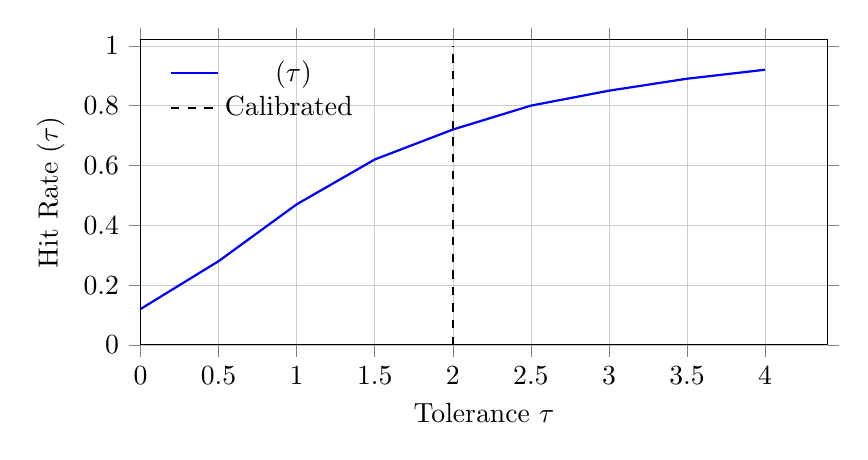
\begin{tikzpicture}
\begin{axis}[
    width=0.85\textwidth,
    height=0.45\textwidth,
    xlabel={Tolerance $\tau$},
    ylabel={Hit Rate $\HR(\tau)$},
    ymin=0, ymax=1.02,
    xmin=0,
    grid=both,
    major grid style={line width=.2pt, draw=gray!40},
    minor grid style={line width=.1pt, draw=gray!20},
    tick align=outside,
    legend style={
        at={(0.03,0.97)},
        anchor=north west,
        draw=none,
        fill=none
    }
]

% --- HR@tau curve (illustrative shape) ---
\addplot[
    thick,
    blue
] coordinates {
    (0.0, 0.12)
    (0.5, 0.28)
    (1.0, 0.47)
    (1.5, 0.62)
    (2.0, 0.72)
    (2.5, 0.80)
    (3.0, 0.85)
    (3.5, 0.89)
    (4.0, 0.92)
};

\addlegendentry{$\HR(\tau)$}

% --- Calibrated tau (example) ---
\addplot[
    dashed,
    thick,
    black
] coordinates {
    (2.0, 0.0)
    (2.0, 1.0)
};

\addlegendentry{Calibrated $\taustar$}

\end{axis}
\end{tikzpicture}

\caption{
Illustrative HR@$\tau$ response surface as a function of tolerance.
The curve shows the monotone increase in hit rate as the acceptable error band
widens, with diminishing marginal gains beyond moderate tolerance levels.
The calibrated tolerance $\taustar$ is selected within a stable region of the
response surface, balancing coverage improvement against tolerance inflation.
}
\label{fig:hrtau_response_surface}
\end{figure}

\subsection{Implications for readiness assessment}
\label{subsec:response_surface_readiness}

Framing \HRtau{} as a response surface clarifies that tolerance-based evaluation
does not yield a single truth but a family of conclusions indexed by $\tauv$.
Readiness judgments based on \HRtau{} therefore depend on where evaluation is
conducted along this surface.

This perspective motivates the use of sensitivity diagnostics and principled
calibration rules.
Rather than fixing $\tauv$ arbitrarily, practitioners can examine how readiness
claims evolve across tolerance values and select reference points that are stable,
interpretable, and aligned with operational standards.

The next section operationalizes this view by introducing grid-based sensitivity
analysis for \HRtau{}, making tolerance dependence explicit and inspectable.